\chapter{Grundlagen}

\section{Historie}

Seit dem Beginn des Industriezeitalters um 1800, welches mit der Mechanisierung (Industrie 1.0) startete, befindet sich die Industrie in einem stetigen Wandel. Sie entwickelte sich um 1900 durch die Massenproduktion zur Industrie 2.0 und in den 1970er Jahren durch die Automatisierung zur Industrie 3.0. Die Einteilung der Industriezeitalter ist durch tiefgreifende Veränderungen im technologischen Fortschritt möglich, welche auch als industrielle Revolution bezeichnet werden. Aktuell befinden wir uns in der Phase der 4. industriellen Revolution.

\subsection{1. industrielle Revolution}

Die 1. industrielle Revolution fand mit der Erfindung der Dampfmaschine statt. Sie ermöglichte es Eisenbahnen und Dampfschiffe sowie verschiedene Maschinen im Kohleabbau oder in Textilfabriken anzutreiben und trug massiv zur Industrialisierung und der Entstehung der Industrie 1.0 bei. Nach und nach wurden immer mehr Produktionsanlagen errichtet und somit Arbeitsplätze in Infrastruktur, Textilfabriken, Häuserbau, Kohleabbau und anderen Bereichen geschaffen.

\subsection{2. industrielle Revolution}

Die Erforschung der Elektrizität im 19. Jahrhundert war der Auslöser der 2. industriellen Revolution. Nachdem ab 1830 die Gesetze der Elektrotechnik bekannt waren, fand die Elektrizität eine breite Anwendung in der Industrie und im Alltag. Im Jahr 1913 führte Henry Ford das Fließband in der Automobilbranche ein. Im Zuge dessen musste jeder Arbeiter nur noch einen Arbeitsschritt erledigen, welches einerseits die Produktion wesentlich beschleunigte und eine Massenproduktion ermöglichte und andererseits eine hohe Spezialisierung der einzelnen Arbeitskräfte für ihre bestimmte Aufgabe erforderte.

Außerdem wurde es durch die Luftfahrt möglich Produkte wie Autos, Kleidung und Lebensmittel über Kontinente hinweg immer schneller zu transportieren und zu handeln.

\subsection{3. industrielle Revolution}

Die 3. industrielle Revolution fand in den 1970er Jahren statt. Sie ist durch eine sukzessive (Teil-) Automatisierung der Prozesse und durch den Einzug der IT in die Industrie- und Verbraucherwelt geprägt. In den 1940er Jahren wurden die ersten Rechenmaschinen und programmierbare Steuerungen in Unternehmen eingesetzt. In den 1970er Jahren zog der Computer auch in den Privatbereich ein, wurde zunehmend beliebter und schaffte einen neuen Industriezweig. Der Fertigungsprozess in Fabriken wurde mehr und mehr von Maschinen übernommen.

Durch den zunehmenden Einsatz von IT in Unternehmen entstand immer mehr Kommunikation zwischen Menschen und Maschinenn. Diese Kommunikation und die anfallenden Daten wurden jedoch nur unternehmensintern verarbeitet. Es gab nur wenige Schnittstellen nach außen.

\begin{figure}[h]
  \centering
  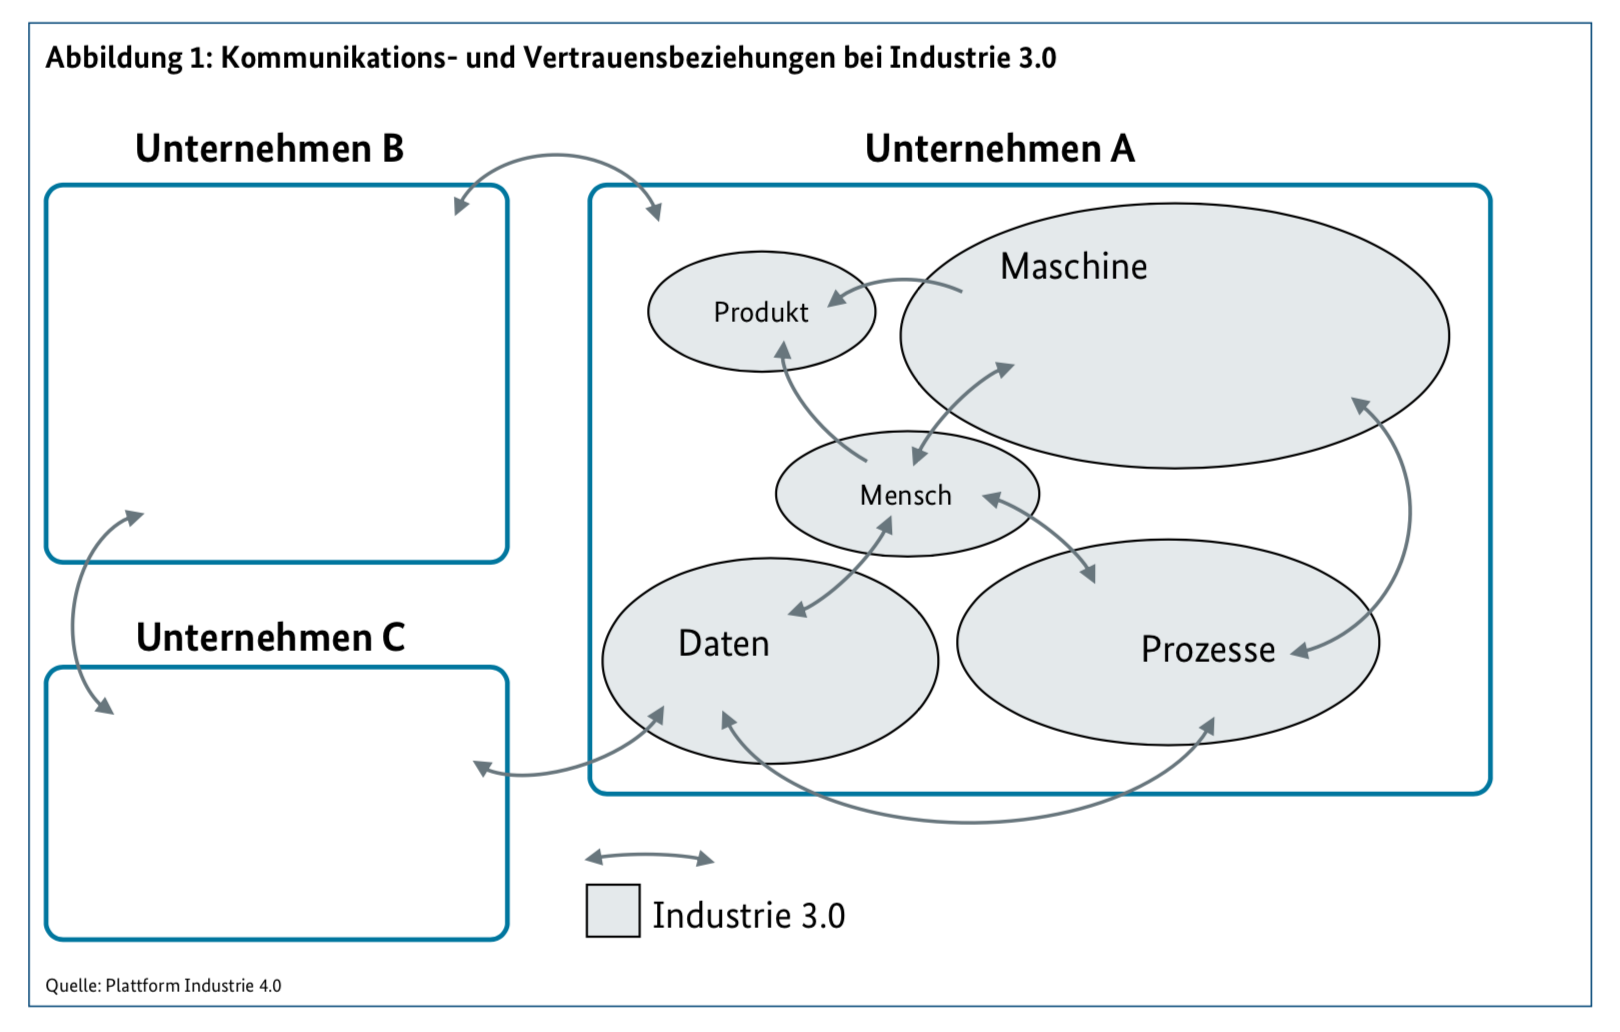
\includegraphics[width=15cm]{kommunikationsbeziehungen-i30}
  \caption{Kommunikationsbeziehungen in einer Industrie 3.0 Umgebung - TODO ref. sichere unternehmensübergreifende Kommunikation}
  \label{Kap2:Industrie3.0-Kommunikation}
\end{figure}

\clearpage

\subsection{4. industrielle Revolution}

Das Ende des 20. Jahrhunderts gilt als der Beginn der 4. industriellen Revolution. Das Kennzeichen dieser Phase ist die zunehmende Digitalisierung. Mit ihr geht die technische Vernetzung physischer Gegenstände, dem \ac{IOT}, einher. Mehr und mehr Geräte oder Gegenstände besitzen die Möglichkeit aktiv durch Datenaustausch oder passiv z. B. mit Hilfe eines Bar- oder QR-Codes mit der digitalen Welt zu kommunizieren und somit eine fortschreitende Automatisierung sowie Individualisierung zu ermöglichen.

Im Gegensatz zur Industrie 3.0 sollen Maschinen autonom, auch über Unternehmensgrenzen hinweg, miteinander kommunizieren können um gesamte Geschäftsprozesse zu übernehmen. Dies setzt eine Öffnung der Unternehmen nach außen voraus.

\begin{figure}[h]
  \centering
  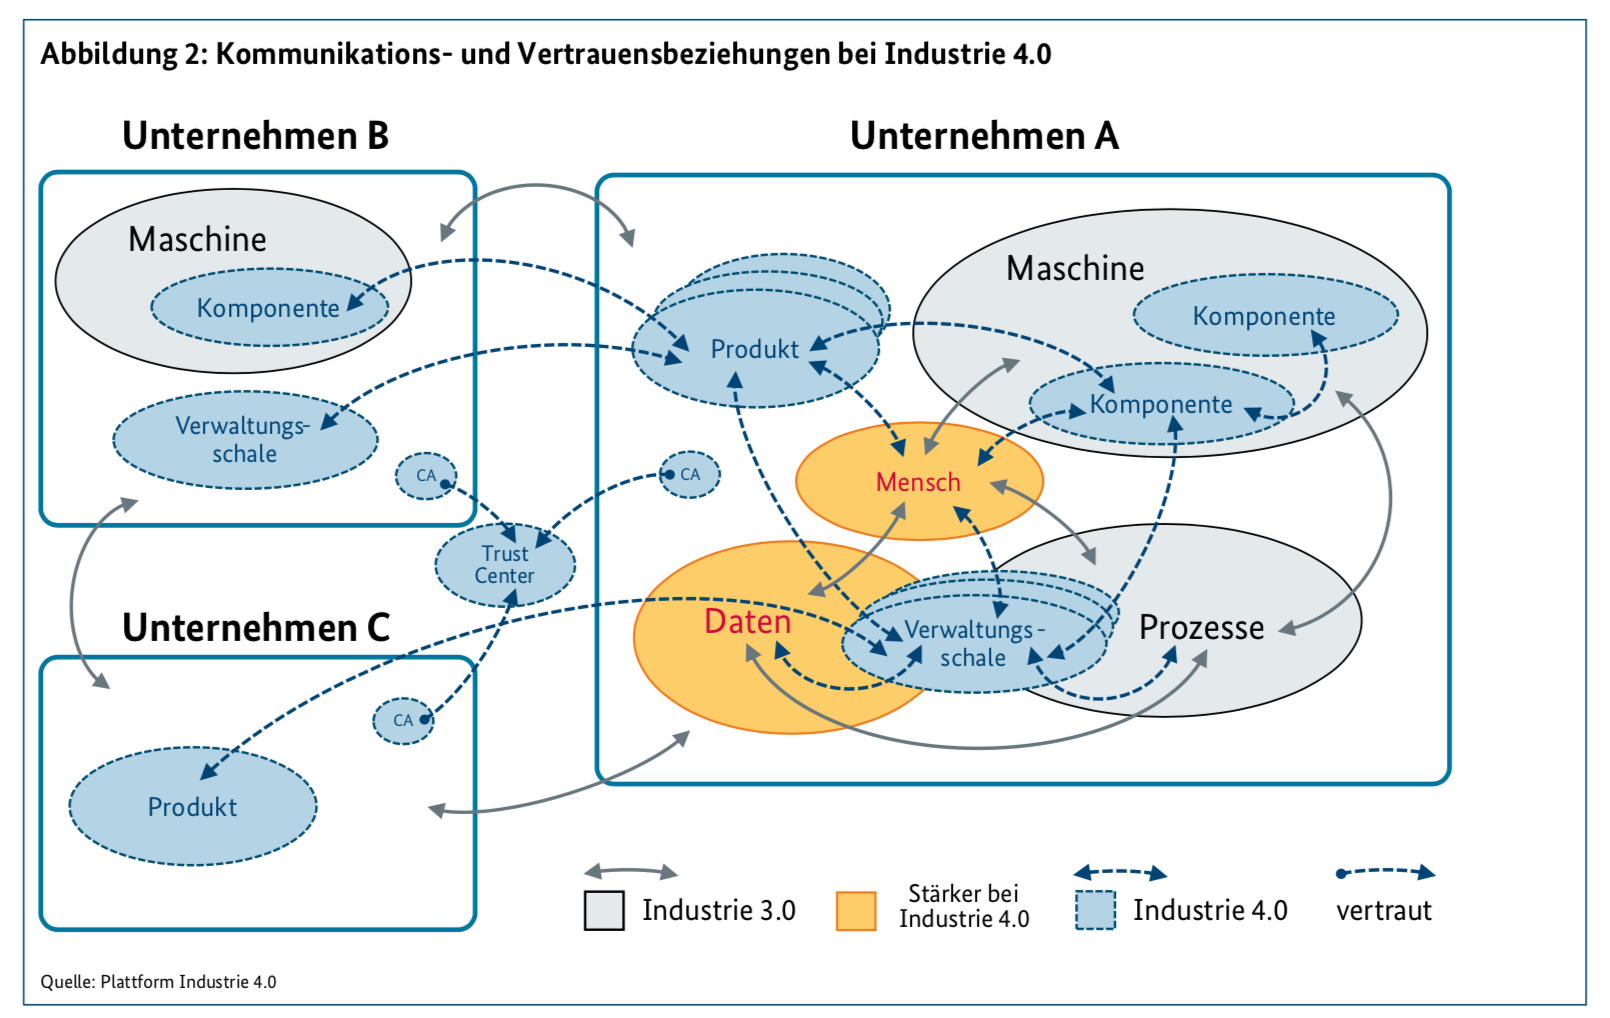
\includegraphics[width=15cm]{kommunikationsbeziehungen-i40}
  \caption{Kommunikationsbeziehungen in einer Industrie 4.0 Umgebung - TODO ref. sichere Unternehmensübergreifende Kommunikation}
  \label{Kap2:Industrie4.0-Kommunikation}
\end{figure}

\clearpage

Diese Entwicklung erzeugt durch die ständige Kommunikation eine ernome Menge an Daten, welche den Anforderungen der IT-Sicherheit gerecht werden müssen, um Verbraucher und Unternehmen zu schützen.

\section{Aktueller Stand der Technik}
Die Entwicklung der Industrie zu ihrer vierten Revolution ist ein stetiger, nicht abgeschlossener Prozess. Aktuell werden die ersten Smart Factories der Industrie errichtet und erste smarte Einkaufsmöglichkeiten, wie Amazon Go und TODO - siehe Trumpf, für den Endverbraucher geschaffen. Diese Fabriken und Filialen stellen die ersten ihrer Art dar und dienen als Prototypen. Das Ziel des Wandels in der Strukturierung und Organisation der Produktion in Unternehmen ist eine immer weitere Automatisierung der Prozessabwicklung bis hin zu autonom arbeitenden Fabriken.

TODO alte Maschinen alte Protokolle

\section{Industrie 4.0}

Der Grundgedanke von Industrie 4.0 ist die flächendeckende Vernetzung von Informations- und Kommunikationstechnik zu einem Internet der Dinge, Dienste und Daten (Spath, 2014 - TODO ref.). 

Dies beinhaltet die Vernetzung der Komponenten auf horizontaler und vertikaler Ebene. Die horizontale Ebene beschreibt die Beteiligten eines Geschäfts- bzw. Produktionsprozesses: Einkauf, Lieferanten, Prouktionsplanung, Logistik, Sequenzierung und Lagerverwaltung. In der vertikalen Ebene befinden sich die verschiedenen Systeme, welche während des Fertigungsprozesses beteiligt sind: ERP, MES und Shopfloor IT.

Die Vernetzung aller Systeme stellt den Übergang einer linearen Prozesskette hin zu einem vermaschten Netzwerk, in dem jede Komponente mit dem gesamten Netzwerk kommunizieren kann, dar.

\begin{figure}[h]
  \centering
  \includegraphics[width=10cm]{horizontaleVertikaleIntegration}
  \caption{horizontale und vertikale Integration - TODO ref. HP industry-of-things siehe bookmark}
  \label{Kap2:horizontale und vertikale Integration}
\end{figure}

\clearpage

\subsection{\ac{RAMI4.0}}
TODO - notwendig? Schichtenmodell, Darstellung eines Assets. nur kurze Beschreibung? wenig Bezug zur Netzwerkkommunikation. Smart Sensors, Kommunikationsfähigkeit eines Assets (aktiv,passiv)

\subsection{Automatisierungspyramide}
Die Automatisierungspyramide stellt die beteiligten Systeme und Softwarekomponenten eines automatisierten Prozesses systematisch dar. Diese beginnen, ausgehend vom Kundenauftrag und der betriebswirtschaftlichen Planung der Produktion auf der Unternehmensebene im \ac{ERP} System. Die Ergebnisse der Planung werden an das \ac{MES} übergeben, welches die verschiedenen Fertigungs- oder Logistikaufträge generiert. Die Aufträge werden anschließend auf der Prozessleit- (\ac{SCADA}), Steuerungs- (\ac{SPS}) und Feldebene (Ein-/Ausgangssignale) bearbeitet.

\begin{figure}[h]
  \centering
  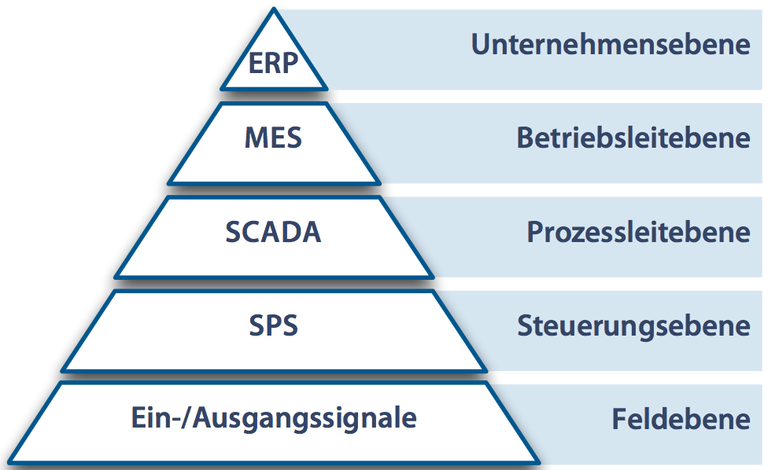
\includegraphics[width=10cm]{automatisierungspyramide}
  \caption{Automatisierungspyramide - TODO ref. Langmann,2004}
  \label{Kap2:Automatisierungspyramide}
\end{figure}

\clearpage

Während die oberen Schichten der Pyramide (\ac{ERP} und \ac{MES}) durch Standardkomponenten bzw. -software der IT realisiert werden, zählen die unteren Schichten (Prozessleit- bis Feldebene) zur Automatisierung, welche die Steuerung und Kontrolle der technischen Anlagen übernimmt. Diese werden auch als Shop-Floor-Ebene bezeichnet. Sie sind durch spezielle Hard- und Softwarelösungen umgesetzt. Die Kommunikation dieser Systeme ist u. a. für spezielle Anwendungsfälle wie harte Echtzeitreaktionszeiten mit Verzögerungen <1ms ausgelegt. Die Integration von Sicherheitsmaßnahmen bei der Kommunikation dieser Systeme stellt oft eine große Herausforderung dar.

\section{Grundprinzipien der sicheren Kommunikation}
\subsection{Vertraulichkeit/Zugriffsschutz}
\subsection{(Daten-)Integrität/Änderungsschutz}
\subsection{Authentizität/Fälschungsschutz}
\subsection{Verbindlichkeit/Nichtabstreitbarkeit}
\subsection{Anonymität}

TODO - Industrie 4.0 beinhaltet durch die Unternehmensübergreifende Kommunikation außerdem den rechtlichen Rahmen, welcher bei Nichteinhaltung von Verträgen bzgl. Verfügbarkeit, Integrität und Vertraulichkeit gelten kann.

\section{sichere Kommunikation in Industrie 4.0}
Im Gegensatz zur I3.0, in welcher Daten auf lokaler Ebene oder zwischen einzelnen internen Unternehmensebenen ausgetauscht wurden, stellt in der I4.0 der Austausch von Daten und Informationen über Unternehmensgrenzen hinweg eine wesentliche Herausforderung dar. Dabei findet die Kommunikation nicht mehr über ein Enterprise-Resource-Planning-System (ERP) statt, sondern auch direkt von einer darunterliegenden Ebene, wie z. B. einer Maschine mit ihrem Lieferanten. Durch diese enge Vernetzung können sowohl Menschen, als auch Maschinen die Kommunikationspartner sein.

\subsection{Anforderungen}
\subsection{Komponenten einer I4.0 Architektur}
\subsubsection{Assets}
\subsubsection{Smarte Sensoren}
\subsubsection{TODO}

\subsection{Kommunikationsstrukturen}
\subsubsection{End2End}
\subsubsection{Gateways}
\subsubsection{Publish-Subscribe}
\subsubsection{Kommunikation mit Netzwerk als Partner}